\documentclass[14pt]{extarticle}
\usepackage[utf8]{inputenc}
\usepackage[T1]{fontenc}
\usepackage[polish]{babel}
\usepackage{tabularray}
\usepackage{graphicx} % Required for inserting images
\usepackage{svg}
\usepackage{tikz-timing}
\usepackage{float}

\makeatletter
\renewcommand\paragraph{\@startsection{paragraph}{4}{\z@}%
	% display heading, like subsubsection
	{-3.25ex\@plus -1ex \@minus -.2ex}%
	{1.5ex \@plus .2ex}%
	{\normalfont\normalsize\bfseries}}
\setcounter{secnumdepth}{4}
\makeatother

\graphicspath{ {./images/} }

\setlength{\parindent}{0pt}
\usetikztiminglibrary[new={char=Q,reset char=R}]{counters}

\title{\huge{\textbf{Tura}} \\ \large{Fizyczna implementacja maszyny Turinga}}
\author{Paweł Szymański}
\date{Luty 2026}

\begin{document}
	
	\maketitle
	\tableofcontents
	\newpage
	
	\section{Wstęp}
	Niewątpliwie jednym z najważniejszych osiągnięć ludzkości XX wieku jest wynalazek będący abstrakcyjnym modelem matematycznym. Mowa oczywiście o maszynie Turinga. Dzięki temu rewolucyjnemu wynalazkowi dziś jako ludzkość jesteśmy w stanie automatyzować zaawansowane zagadnienia, jak na przykład obróbka i montaż produktów w fabrykach czy rozwiązywanie skomplikowanych obliczeń matematycznych. Bez maszyn Turinga nie mielibyśmy dziś komputerów, urządzeń tak uniwersalnych i wszechstronnych jak te które znamy, z których korzystamy i z którego najprawdopodobniej czytelnik czyta tę dokumentację. W ramach urzeczywistnienia matematycznego modelu maszyny Turinga powstał projekt ,,Tura'', którego zadaniem jest fizyczna implementacja pewnego modelu maszyny. Z racji, iż podstawowy model zakłada nieograniczoną długość taśmy, implementajca maszyny jako takiej nie jest możliwa. Jednak pewien podzbiór maszyn zakłada skończoną długość taśmy. Tym modelem jest maszyna Turinga ograniczona liniowo. Implementowany model, w celu uproszczenia elektronicznych układów, dodatkowo posiada własność akceptującego stanu zatrzymującego.
	
	\section{Opis zastosowanego modelu}
	Definicja maszyny Turinga $M$ jest następująca:
	
	\[
	M = (Q, \Gamma, \Sigma, \delta, q_0, B, F),
	\]
	gdzie:
	\begin{itemize}
		\item $Q$ - zbiór stanów,
		\item $\Gamma$ - alfabet taśmy,
		\item $\Sigma$ - alfabet słowa wejściowego, $\Sigma \subseteq \Gamma$,
		\item $\delta$ - funkcja przejścia, $\delta: Q \times \Gamma \rightarrow Q \times \Gamma \times D$, gdzie $D$ jest zbiorem możliwych ruchów głowicy maszyny, $D = \{L, R\},$
		\item $q_0$ - stan początkowy, $q_0 \in Q$,
		\item $B$ - symbol pusty, $B \in \Gamma \backslash \Sigma$,
		\item $F$ - zbiór stanów akceptujących.
	\end{itemize}
	Żeby znaleźć jakieś intuicyjne wyobrażenie jak taka maszyna może wyglądać i funkcjonować możemy wyobrazić sobie skrzynkę, w której zamknięty jest układ sterujący urządzeniem oraz przede wszystkim przechowujący jego obecny stan. Obok skrzynki umieszczona jest taśma z symbolami. Ma ona swój początek z jednej strony, jednak z drugiej nie ma końca - jest jednostronnie nieskończona. Taśmę i skrzynkę łączy głowica - czyta ona lub nadpisuje jeden symbol na taśmie oraz przesuwa się po niej. Na początku działania maszyny głowica znajduje się nad skrajnym symbolem taśmy.
	\newline \newline
	Działanie takiej maszyny można porównać do następującej sekwencji czynów:
	\begin{enumerate}
		\item Głowica odczytuje symbol $s \in \Gamma$ z taśmy.
		\item Skrzynka na podstawie obecnego stanu $q \in Q$ oraz $s$ oblicza nowy stan, symol i kierunek przesunięcia głowicy za pomocą funkcji przejścia:  $\delta(q,s) = (q', s', d)$.
		\item Skrzynka zmienia obecny stan z $q$ na $q'$.
		\item Głowica nadpisuje symbol na taśmie $s$ na $s'$, po czym przesuwa się o jeden symbol się zgodnie z kierunkiem $d$.
		\item Sekwencja ta jest powtarzana dopóty, dopóki maszyna nie osiągnie stanu akceptującego.
	\end{enumerate}
	
	\begin{figure}[h!]
		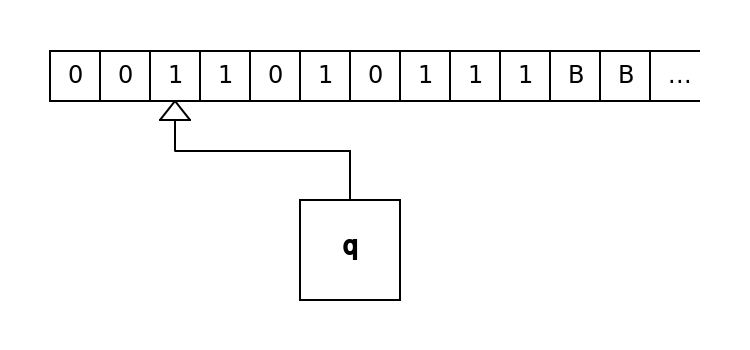
\includegraphics[width=\linewidth]{mt.png}
		\caption{Przykładowa wizualizacja maszyny Turinga}
		\label{fig:examplemtmeaning}
	\end{figure}
	
	Fizyczne urządzenie cechuje się dodatkowo ograniczoną długością taśmy oraz jednym stanem akceptującym zatrzymującym działanie maszyny. Formalnie ograniczoną długość taśmy można uzyskać poprzez wstawienie wartowników na jej początku oraz końcu, jednak te działanie pozostawione jest dla użytkownika maszyny do samodzielnej implementacji. Zaś stan akceptujący zatrzymujący działanie maszyny oznacza, że $F$ ma dokładnie jeden stan akceptujący $q_A$, po którego osiągnięciu urządzenie zatrzymuje pracę. 
	
	\section{Model Działania}
	\subsection{Opis Ogólny}
	Działanie maszyny w skrócie opiera się o zaprogramowanie urządzenia, wykonanie obliczeń i pobranie wyniku.
	\begin{itemize}
		\item Programowanie odbywa się poprzez zapisanie wejściowej zawartości taśmy oraz funkcji przejścia w trzech blokach pamięci (bloku symboli taśmy, bloku funkcji przejścia symbolu tasmy oraz bloku funkcji przejścia stanu). 
		\item Wykonanie obliczeń to uruchomienie urządzenia i pozostawienie w działaniu do czasu osiągnięcia stanu akceptującego.
		\item Pobranie wyniku jest odczytem zawartości taśmy po zakończeniu działania maszyny.
	\end{itemize}
	
	\subsection{Opis Szczegółowy}
	Opis szczegółowy wchodzi już w fizyczną implementację urządzenia. Jego celem jest staranny opis modułów, sygnałów, ich wzajemnej interakcji oraz dokładne wytłumaczenie działania maszyny. Opis w znacznej mierze opiera się o schematy KiCad i korzysta ze stosowanych w nich oznaczeń oraz nazw.
	
	\subsubsection{Moduły}
	Maszyna została podzielona na 11 modułów w celu oznakowania jednostek odpowiedzialnych za poszczególne funkcje. Moduły w schematach KiCad zostały otoczone ciemnożłółtymi ramkami i podpisane niebieskim tekstem lub jedynie podpisane niebieskim tekstem w przypadku modułów jednoelementowych.
	\begin{description}
		\item[\texttt{TAPE}] -- Blok pamięci symulujący taśmę. Każda komórka pamięci reprezentuje jeden symbol taśmy. Pojedynczy symbol taśmy składa się z 7 bitów;
		\item[\texttt{TAPE SYMBOL REGISTER}] -- Rejestr przechowujący jeden symbol taśmy. Jest on potrzebny do chwilowego przechowania odczytanego symbolu na czas zapisu nowego do \texttt{TAPE};
		\item[\texttt{SYMBOL TRANSLATOR}] -- Blok pamięci symulujący funkcję przejścia dla zadanego symbolu oraz stanu zwracający wynik w formie symbolu taśmy (7 bitów) oraz kierunku ruchu głowicy (1 bit);
		\item[\texttt{STATE TRANSLATOR}] -- Blok pamięci symulujący funkcję przejścia dla zadanego symbolu oraz stanu zwracający wynik w formie stanu (8 bitów);
		\item[\texttt{STATE REGISTER}] -- Rejestr przechowujący obecny stan maszyny;
		\item[\texttt{HEADER POSITION}] -- Zbiór liczników binarnych z możliwością inkrementacji oraz dekrementacji reprezentujący usytuowanie głowicy na taśmie (wskazuje obecnie wybrany symbol w \texttt{TAPE});
		\item[\texttt{HEADER POSITION DIRECTION DISASSEMBLY}] -- Prosty multiplekser sygnału zmiany wartości \texttt{HEADER POSITION} w zależności od kierunku zmiany;
		\item[\texttt{HEADER POSITION CLOCK SYNCHRONIZATION}] -- Bramka AND synchronizująca sygnał zmiany wartości \texttt{HEADER POSITION} z zegarem;
		\item[\texttt{STEP EXECUTION STATE REGISTER}] -- Rejestr przechowujący obecny stan wykonywania ruchu maszyny. Ze względu na brak praktycznego rozwiązania jednoczesnego odczytu i zapisu symbolu taśmy, przeprowadzenie przejścia zostało podzielone na dwa ruchy rozdzielające te operacje; stąd dwa stany wykonania ruchu;
		\item[\texttt{IN-PROGRAM CONTROL LINES BUFFERS}] -- Zestaw buforów oddzielający kontrolne linie sygnałowe generowane przez interfejs zewnętrzny od tych wewnęrznych;
		\item[\texttt{IN-OPERATION CONTROL LINES BUFFER}] -- Bufor oddzielający wewnętrzne linie kontrolne od tych generowanych przez urządzenie podczas pracy; %Rozdzielenie to jest potrzebne w celu umożliwienia programowania maszyny (dostępu sygnałów zewnętrznych do wewnętrznych);
	\end{description}
	
	\subsubsection{Sygnały}
	Oznaczenie sygnałów jest takie same jak oznaczenia zastosowane w schematach KiCad. Sygnały z $\overline{\texttt{poprzeczką nad nazwą}}$ oznaczają, że sygnał jest aktywny dla niskiego poziomu, zaś nieaktywny dla wysokiego.
	%Część sygnałów nie ma bezpośredniego zastosowania podczas pracy maszyny, jednak są one potrzebne do jej programowania i odczytu wyniku pracy. Te sygnały znajdują się w interfejsie zewnętrznym, który został opisany w następnym podrozdziale. 
	\newline \newline
	\textbf{Lista sygnałów}:
	\begin{description} 
		\item[\texttt{D\textsubscript{0...7}}] -- Magistrala danych używana do programowania i odczytu  danych z maszyny;
		\item[\texttt{S\textsubscript{0...6}}] -- Magistrala symbolu taśmy;
		\item[\texttt{SR\textsubscript{0...6}}] -- Magistrala symbolu taśmy zapisanego w \texttt{TAPE SYMBOL REGISTER};
		\item[\texttt{Q\textsubscript{0...7}}] -- Magistrala stanu;
		\item[\texttt{QR\textsubscript{0...7}}] -- Magistrala stanu zapisanego w \texttt{STATE REGISTER};
		\item[\texttt{H\textsubscript{0...15}}] -- Magistrala z wartością licznika \texttt{HEADER POSITION};
		\item[\texttt{CLK}] -- Sygnał zegarowy wyznaczający rytm pracy; każda zmiana sygnału ze stanu niskiego do wysokiego powoduje przejście \texttt{STEP EXECUTION STATE REGISTER} do następnego stanu; działa pod warunkiem aktywnego sygnału \texttt{CLK\_EN};
		\item[\texttt{CLK\_EN}] -- Kontroluje dopływ sygnału \texttt{CLK} do \texttt{STEP EXECUTION STATE REGISER};
		\item[\texttt{DIR}] -- Ustala kierunek zmiany wartości \texttt{HEADER POSITION}. Wysoki stan sygnału znaczy inkrementację, niski stan dekrementację;
		\item[\texttt{HP\_EN}] -- Dopuszcza możliwość zmiany wartości \texttt{HEADER POSITION};
		\item[\texttt{HP\_EN\_CLK}] -- sygnał \texttt{HP\_EN} zsynchronizowany z zegarem (\texttt{CLK}): $\texttt{HP\_EN\_CLK} = \texttt{HP\_EN} \cdot \texttt{CLK}$; synchronizuje zmianę wartości \texttt{HEADER POSITION} z zegarem;
		\item[\texttt{DIR\_UP}] -- Decyduje o inkrementacji wartości \texttt{HEADER POSITION}; działa przy przejściu ze stanu niskiego do wysokiego;
		\item[\texttt{DIR\_DOWN}] -- Decyduje o dekrementacji wartości \texttt{HEADER POSITION}; działa przy przejściu ze stanu niskiego do wysokiego;
		\item[$\overline{\texttt{RESET}}$] -- Resetuje urządzenie, czyli ustawia \texttt{STEP EXECUTION STATE REGISTER} do stanu $0$ oraz ustawia wartość \texttt{HEADER POSITION} na $0$;
		\item[$\overline{\texttt{PROGRAM}}$] -- Ustala tryb pracy. Poziom niski sygnału oznacza tryb programowania maszyny, poziom wysoki zaś tryb wykonywania programu;
		\item[\texttt{PROGRAM}] -- Przeciwieństwo sygnału $\overline{\texttt{PROGRAM}}$; sygnał ten jest równoważny $\overline{\texttt{OPERATE}}$ -- podany został jedynie dla czytelności schematu;
		\item[$\overline{\texttt{OPERATE}}$] -- Przeciwieństwo sygnału $\overline{\texttt{PROGRAM}}$. Niski poziom oznacza pracę urządzenia;
		\item[\texttt{DDIR}] -- Ustala kierunek przepływu danych z wewnętrznych modułów wybranych sygnałami \texttt{CS\textsubscript{0}}, \texttt{CS\textsubscript{1}} na magistralę \texttt{D\textsubscript{0...7}}. Wysoki poziom sygnału oznacza zapis danych z inteferjsu zewnętrznego do modułów wewnątrz urządzenia. Niski poziom oznacza odczyt;
		\item[\texttt{CS\textsubscript{0}}, \texttt{CS\textsubscript{1}}] -- Kombinacja tych sygnałów wybiera wewnętrzną magistralę, która zostanie połączona z zewnętrzną \texttt{D\textsubscript{0...7}} oraz wewnętrzny moduł do odczytu/zapisu danych z wybranej magistrali (kierunek zależny od \texttt{DDIR});
		\item[$\overline{\texttt{DT}}$] -- Włącza przesył danych między wewnętrznymi modułami a intefrejsem zewnętrznym; aktywny dla niskiego poziomu;
		\item[\texttt{TSR\_WR}] -- Zapisuje dane z magistrali symbolu taśmy \texttt{S\textsubscript{0...6}} do \texttt{TAPE SYMBOL REGISTER}; zapis odbywa się podczas przejścia sygnału ze stanu niskiego do wysokiego;
		\item[\texttt{SR\_WR}] -- Zapisuje dane z magistrali stanu \texttt{Q\textsubscript{0...7}} do \texttt{STATE REGISER}; zapis odbywa się podczas przejścia sygnału ze stanu niskiego do wysokiego;
		\item[\texttt{T\_$\overline{\texttt{OE}}$}] -- Włącza wyjście danych z \texttt{TAPE} na magistralę \texttt{S\textsubscript{0...6}}; aktywny dla niskiego poziomu;
		\item[\texttt{T\_$\overline{\texttt{WE}}$}] -- Włącza zapis danych w \texttt{TAPE} z magistrali \texttt{S\textsubscript{0...6}}; aktywny dla niskiego poziomu;
		\item[\texttt{SYT\_$\overline{\texttt{OE}}$}] -- Włącza wyjście danych z \texttt{SYMBOL TRANSLATOR} na magistralę \texttt{S\textsubscript{0...6}} oraz sygnał \texttt{DIR\_B}; aktywny dla niskiego poziomu;
		\item[\texttt{SYT\_$\overline{\texttt{WE}}$}] -- Włącza zapis danych w \texttt{SYMBOL TRANSLATOR} z magistrali \texttt{S\textsubscript{0...6}} oraz sygnału \texttt{DIR\_B}; aktywny dla niskiego poziomu;
		\item[\texttt{STT\_$\overline{\texttt{OE}}$}] -- Włącza wyjście danych ze \texttt{STATE TRANSLATOR} na magistralę \texttt{Q\textsubscript{0...7}}; aktywny dla niskiego poziomu;
		\item[\texttt{STT\_$\overline{\texttt{WE}}$}] -- Włącza zapis danych w \texttt{STATE TRANSLATOR} z magistrali \texttt{Q\textsubscript{0...7}}; aktywny dla niskiego poziomu;
		\item[\texttt{QR\_$\overline{\texttt{OE}}$}] -- Włącza wyjście danych ze \texttt{STATE REGISTER} na magistralę \texttt{D\textsubscript{0...7}}; aktywny dla niskiego poziomu;
		\item[\texttt{T\_$\overline{\texttt{*E}}$\_E}, \texttt{SYT\_$\overline{\texttt{*E}}$\_E}, \texttt{ST\_$\overline{\texttt{*E}}$\_E}, \texttt{QR\_$\overline{\texttt{OE}}$\_E}] -- Sygnały odpowiadające tym bez sufiksu ,,\texttt{\_E}'', będące połączone z nimi przez bufor \texttt{U18} oraz będące wynikiem dekodera wyboru funkcji \texttt{U19};
		\item[\texttt{T\_$\overline{\texttt{*E}}$\_B}, \texttt{SYT\_$\overline{\texttt{OE}}$\_B}, \texttt{STT\_$\overline{\texttt{OE}}$\_B}, \texttt{DIR\_B}] -- Sygnały odpowiadające tym bez sufiksu ,,\texttt{\_B}'', będące połączone z nimi przez bufor \texttt{U17}. Są one sygnałami generowanymi przez maszynę podczas obliczeń potrzebnymi do poprawnej jej samodzielnej pracy;
		\item[$\overline{\texttt{SYMB\_BUF}}$] -- Włącza przepływ danych z \texttt{TAPE} lub \texttt{SYMBOL TRANSLATOR} (w zależności od wybranego urządzenia sygnałami \texttt{CS\textsubscript{0,1}}) na magistralę \texttt{D\textsubscript{0...7}}; aktywny dla niskiego poziomu;
		\item[$\overline{\texttt{STAT\_BUF}}$] -- Włącza przepływ danych ze \texttt{STATE TRANSLATOR} na magistralę \texttt{D\textsubscript{0...7}}; aktywny dla niskiego poziomu;
		\item[$\overline{\texttt{FINISH\_STATE}}$] -- Informuje o osiągnięciu przez maszynę stanu akceptującego i zarazem zatrzymującego pracę; aktywny dla niskiego poziomu.
		\item[\texttt{SEST\_STATE}] -- Wskazuje obecny stan \texttt{STEP EXECUTION STATE REGISTER};
	\end{description}
	
	\subsubsection{Interfejs zewnętrzny}
	W celu zasilenia urządzenia oraz komunikacji zastosowany został zewnętrzny interfejs w formie złącza krawędziowego. Składa się on z 17 wyjść sterujących oraz informujacych o stanie maszyny, 11 zasilających oraz 16 niepodpiętych do żadnych sygnałów. W sumie daje to 44 wyjścia. Wszystkie wspomniane sygnały (po za \texttt{Vcc} oraz \texttt{Vss}) zostały wyjaśnione w poprzednim podrozdziale. Wyjścia \texttt{Vcc} oraz \texttt{Vss} są wyjściami odpowiednio zasilania i uziemienia. \texttt{Vcc} powinno mieć napięcie +5V względem \texttt{Vss}. \\
	By uniknąć zbyt podobnych oznaczeń, kierunki sygnałów zamiast ,,Wej/Wyj'' zostały oznaczone angielskimi ,,In/Out''.
	\newline \newline
	\textbf{Tabela sygnałów interfejsu:}
	\SetTblrInner{rowsep=4pt}
	\begin{table}[H]
		\centering
		\begin{tblr}{||c|c|c||}
			\hline
			\textbf{Num. wyjścia} & \textbf{Sygnały} & \textbf{Kierunek} \\ \hline
			1-8 & \texttt{D\textsubscript{0...7}} & In/Out \\ \hline
			9 & \texttt{CLK} & In \\ \hline
			10 & $\overline{\texttt{RESET}}$ & In \\ \hline
			11 & $\overline{\texttt{PROGRAM}}$ & In \\ \hline
			12 & \texttt{DDIR} & In \\ \hline
			13-14 & \texttt{CS\textsubscript{0,1}} & In \\ \hline
			15 & $\overline{\texttt{DT}}$ & In \\ \hline
			16 & $\overline{\texttt{FINISH\_STATE}}$ & Out \\ \hline
			17 & \texttt{SESR\_STATE} & Out \\ \hline
		\end{tblr}
		\caption{Lista sygnałów interfejsu zewnętrznego}
		\label{tab:extinterfacetable1}
	\end{table}
	\begin{table}[H]
		\centering
		\begin{tblr}{||c|c|c||}
			\hline
			\textbf{Num. wyjścia} & \textbf{Sygnały} & \textbf{Kierunek} \\ \hline
			19,21,23,25,27 & \texttt{Vcc} & --- \\ \hline
			18,20,22,24,26,28 & \texttt{Vss} & --- \\ \hline
			29-44 & --- & --- \\ \hline
		\end{tblr}
		\caption{Lista sygnałów interfejsu zewnętrznego (cd.)}
		\label{tab:extinterfacetable2}
	\end{table}
	
	Oprócz interfejsu zewnętrznego na urządzeniu znajdują się trzy dodatkowe złącza: J2, J3 i J4. Służą one do odczytu wartości odpowiednio \texttt{TAPE SYMBOL REGISTER}, \texttt{STATE REGISTER} oraz \texttt{HEAD POSITION} (złącza te są podłączone do tych modułów bezpośrednio).
	
	\subsubsection{Programowanie}
	%Mając na uwadze czytelność dokumentacji zdecydowano o opisie stanu sygnałów w czasie w formie wykresu czasowego. Każdy rząd odpowiada konkretnemu sygnałowi; linia w rzędzie zmieniająca się między stanem wysokim a niskim oznacza stan sygnału w czasie. Każda kolumna wykresu przedstawia konkretny odcinek czasowy wraz ze stanami sygnałów w tym czasie. Odcinki nie mają ustalonego konkretnego czasu trwania, ani nie muszą trwać tyle samo, a mają bardziej na zasadzie pokazać kolejność wysłania sygnałów. Sygnały zmieniane są podczas przejść między odcinkami czasowymi. \newline \newline
	Programowanie maszyny odbywa się za pomocą interfejsu zewnętrznego. Dzięki odpowiedniemu wykorzystaniu udostępnionych sygnałów użytkownik jest w stanie manipulować zawartością bloków pamięci \texttt{TAPE}, \texttt{SYMBOL TRANSLATOR} oraz \texttt{STATE TRANSLATOR}.
	%\newline \newline
	\paragraph{Przygotowanie maszyny do programowania}
	W celu rozpoczęcia programowania maszyny należy wpierw ją do tego przygotować. Zadanie to jest dość proste - wystarczy ustawić sygnał $\overline{\texttt{PROGRAM}}$ na niski poziom, po czym puścić puls sygnału $\overline{\texttt{RESET}}$. Wykres czasowy znajduje się na stronie \pageref{fig:programprep}. na rysunku \ref{fig:programprep}.
	
	\paragraph{Programowanie modułu \texttt{TAPE} (taśmy)}
	Programowanie modułu \texttt{TAPE} zaczyna się przygotowaniem go do programowania, czyli wybraniem modułu, z użyciem sygnałów \texttt{CS\textsubscript{0,1}}, ustaleniem kierunku przepływu danych sygnałem \texttt{DDIR} - poziom wysoki dla zapisu - oraz puszczeniem pulsu sygnału $\overline{\texttt{RESET}}$. \\
	Następnie zapis słowa wejściowego taśmy odbywa się w pętli: ustala się sybol do zapisu na magistrali \texttt{D\textsubscript{0...6}} (proszę zwrócić uwagę na indeks 0...6 - symbol ma 7 bitów), aktywuje się przesył danych (w tym przypadku zapis) do modułu pulsem sygnału  $\overline{\texttt{DT}}$ oraz wysła się dwa pulsy zegara \texttt{CLK} w celu przejścia do następnej komórki pamięci przechowującej zawartość taśmy. Wykres czasowy znajduje się na stronie \pageref{fig:programtape}. na rysunku \ref{fig:programtape}.
	
	\paragraph{Programowanie modułu \texttt{SYMBOL TRANSLATOR}}
	Podobnie jak w przypadku programowania \texttt{TAPE}, \texttt{SYMBOL TRANSLATOR} również należy przygotować do programowania. W tym celu trzeba wybrać jedynie kierunek \texttt{DDIR} oraz puścić puls sygnału $\overline{\texttt{RESET}}$. \\
	Zapis pojedynczej wartości funkcji przejścia z wynikiem w postaci symbolu oraz kierunku przesunięcia głowicy jest bardziej skomplikowany w porównaniu do zapisu pojedynczego symbolu taśmy. Główny problem leży w określeniu, która wartość funkcji ma zostać wgrana do modułu, czyli która komórka pamięci ma być zapisana. Aby to sprecyzować należy dokonać zapisu w dwóch rejestrach, które bezpośrednio określają wskazywane miejsce w pamięci: \texttt{TAPE SYMBOL REGISTER} oraz \texttt{STATE REGISTER}. Te dwa rejestry odpowiadają argumentom funkcji przejścia: stanowi oraz symbolowi. \\
	%Każdy z tych rejestrów ma nadpisywaną swoją zawartość podczas kolejnych pulsów zegara \texttt{CLK}. \\
	Zatem, żeby wskazać miejsce w pamięci modułu \texttt{SYMBOL TRANSLATOR} do którego należy zapisać wartość, trzeba wpierw wysłać symbol będący jednym z argumentów funkcji przejścia na magistralę \texttt{D\textsubscript{0...6}}, wybrać wewnętrzną magistralę \texttt{S\textsubscript{0...6}} sygnałami \texttt{CS\textsubscript{0,1}} oraz wysłać puls zegara w celu zapisania wartości magistrali w \texttt{TAPE SYMBOL REGISTER}. Następnie trzeba wysłać stan będący drugim z argumentów funkcji przejścia na magistralę \texttt{D\textsubscript{0...7}}, wybrać wewnętrzną magistralę \texttt{Q\textsubscript{0...7}} sygnałami \texttt{CS\textsubscript{0,1}} oraz wysłać puls zegara w celu zapisania wartości magistrali w \texttt{STATE REGISTER}. \\
	Po tym miejsce w pamięci modułu \texttt{SYMBOL TRANSLATOR} jest wybrane i można przystąpić do zapisu symbolu oraz kierunku wartości funkcji przejścia. Osiąga się to za pomocą wyboru modułu sygnałami \texttt{CS\textsubscript{0,1}}, umieszczeniu danych do zapisu na magistrali \texttt{D\textsubscript{0...7}} oraz puszczeniem pulsu sygnału. \\
	W przypadku programowania wartości funkcji dla argumentu ze stanem akceptującym po wykonaniu zapisu do \texttt{STATE REGISTER} należy puścić puls sygnału $\overline{\texttt{RESET}}$ w celu wyjścia maszyny ze stanu zatrzymania pracy (zatrzymania wpływu zegara na przejścia między staniami \texttt{STEP EXECUTION STATE REGISTER}). Jednak można zauważyć, że programowanie tych przejść nie ma sensu ze względu na zatrzymanie pracy urządzenia zaraz po przejściu do stanu akceptującego. $\overline{\texttt{DT}}$. \\
	Wykres czasowy znajduje się na stronie \pageref{fig:programsymbol}. na rysunku \ref{fig:programsymbol}.
	
	\paragraph{Programowanie modułu \texttt{STATE TRANSLATOR}}
	Programowanie \texttt{STATE TRANSLATOR} odbywa się w sposób bardzo zbliżony do \texttt{SYBMOL TRANSLATOR}. Wpierw należy przygotować moduł do programowania co dzieje się poprzez ustawienie kierunku sygnałem \texttt{DDIR} oraz puszczenie pulsu sygnału $\overline{\texttt{RESET}}$. \\
	Zapis pojedynczej wartości funkcji przejścia z wynikiem w postaci stanu wymaga dokładnie tego samego procesu wybrania komórki pamięci w \texttt{STATE TRANSLATOR} co w \texttt{SYMBOL TRANSLATOR}. Z tego tytułu opis tego zadania nie został tu omówiony (jednak wciąż znajduje się on na wykresie czasowym). \\
	Po wybraniu miejsca w pamięci modułu \texttt{STATE TRANSLATOR} następuje zapis stanu wartości funkcji przejścia: wybierany jest moduł sygnałami \texttt{CS\textsubscript{0,1}}, umieszczana jest wartość na magistrali \texttt{D\textsubscript{0...7}} oraz puszczony zostaje puls sygnału $\overline{\texttt{DT}}$ w celu zapisania danych w pamięci. Wykres czasowy znajduje się na stronie \pageref{fig:programstate}. na rysunku \ref{fig:programstate}.
	\newline \newline
	Po wykonaniu powyższych czynności, tj. zaprogramowaniu modułów \texttt{TAPE}, \texttt{SYMBOL TRANSLATOR} oraz \texttt{STATE TRANSLATOR} urządzenie jest gotowe do wykonania zapisanego programu.
	
	\paragraph{Wykresy czasowe}
	Poniżej znajdują się wykresy czasowe uprzednio opisanych czynności. \\
	\begin{figure}[H]
		\begin{tikztimingtable}[
			timing/slope=0.1,
			timing/coldist=10pt,
			xscale=2,yscale=2,
			thick
			]
			$\overline{\texttt{PROGRAM}}$	& HLLLLLLLLLLLLLLLLL \\
			$\overline{\texttt{RESET}}$		& HHLHHHHHHHHHHHHHHH \\		
			\extracode
			\begin{pgfonlayer}{background}
				\begin{scope}[gray,semitransparent,semithick]
					\vertlines{1,...,17}
				\end{scope}
				\begin{scope}[gray,semitransparent,semithick]
					\horlines[dotted]{}
				\end{scope}
				\foreach \n in {1,2,...,\twidth}
				\draw (\n-0.5,-\nrows-.8)
				node [below,inner sep=2pt] {\scalebox{.75}{\tiny\n}};
			\end{pgfonlayer}
		\end{tikztimingtable}
		\caption{Wykres czasowy przygotowania maszyny do programowania.}
		\label{fig:programprep}
	\end{figure}
	Na wykresie czasowym przygotowania maszyny do programowania kolumna 2 przedstawia przejście sygnału $\overline{\texttt{PROGRAM}}$ do stanu niskiego, kolumna 3 przedstawia puls sygnału $\overline{\texttt{RESET}}$. Późniejsze kolumny utrzymują stany sygnałów; zostały umieszczone w celach estetycznych wykresu, podobnie jak ten tekst, który służy częściowemu wypełnieniu pustego miejsca do końca tej strony.
	\newpage
	
	\begin{figure}[H]
		\begin{tikztimingtable}[
			timing/slope=0.1,
			timing/coldist=10pt,
			xscale=2,yscale=2,
			thick
			]
			$\overline{\texttt{RESET}}$		& HLHHHHHHHHHHH;[dotted]HHH;HH \\
			\texttt{CS\textsubscript{1}}	& ULLLLLLLLLLLL;[dotted]LLL;LU \\
			\texttt{CS\textsubscript{0}}	& ULLLLLLLLLLLL;[dotted]LLL;LU \\
			\texttt{DDIR}					& UHHHHHHHHHHHH;[dotted]HHH;HU \\
			\texttt{D\textsubscript{0...6}}	& UU DDDDD{}DDDDD{};[dotted]DDDDD{}; U \\
			$\overline{\texttt{DT}}$		& HH HLHHH  HLHHH  ;[dotted]HLHHH; H \\
			\texttt{CLK}					& HH HHLHL  HHLHL  ;[dotted]HHLHL; H \\
			\extracode
			\begin{pgfonlayer}{background}
				\begin{scope}[gray,semitransparent,semithick]
					\vertlines{1,...,17}
				\end{scope}
				\begin{scope}[darkgray,semitransparent,thick]
					\vertlines{2,7,12,17}
				\end{scope}
				\begin{scope}[gray,semitransparent,semithick]
					\horlines[dotted]{}
				\end{scope}
				\foreach \n in {1,2,...,\twidth}
				\draw (\n-0.5,-\nrows-5.8)
				node [below,inner sep=2pt] {\scalebox{.75}{\tiny\n}};
			\end{pgfonlayer}
		\end{tikztimingtable}
		\caption{Wykres czasowy programowania \texttt{TAPE}.}
		\label{fig:programtape}
	\end{figure}
	Na wykresie czasowym programowania \texttt{TAPE} kolumny 1-2 reprezentują przygotowanie \texttt{TAPE} do programowania. 2-6 i 7-11 przedstawiają dwa pojedyncze zapisy symboli do dwóch kolejnych komórek pamięci w \texttt{TAPE}. Sygnały w kolumnach 13-17 zostały wykropkowane w celu wyeksponowania wielokrotnego powielenia operacji zapisu symbolu.
	\newpage
	
	\begin{figure}[H]
		\begin{tikztimingtable}[
			timing/slope=0.1,
			timing/coldist=10pt,
			xscale=1.714,yscale=2,
			thick
			]
			$\overline{\texttt{RESET}}$		& HLHHHHHHHHHH;[dotted]HHHHHHH;HH \\
			\texttt{CS\textsubscript{1}}	& UU LLL HHH LLL;[dotted] LLL HHH LLL; U \\
			\texttt{CS\textsubscript{0}}	& UU HHH LLL HHH;[dotted] HHH LLL HHH; U \\
			\texttt{DDIR}					& UHHHHHHHHHHH;[dotted]HHHHHHH;HU \\
			\texttt{D\textsubscript{0...7}}	& UU DDD{wartość \texttt{TSR}}DDD{wartość \texttt{SR}}DDD{wartość \texttt{SYT}};[dotted]DDD{wartość \texttt{TSR}}DDD{wartość \texttt{SR}}DDD{wartość \texttt{SYT}}; U \\
			$\overline{\texttt{DT}}$		& HH HHH HHH HLH;[dotted]HHH HHH HLH; H \\
			\texttt{CLK}					& HH HLH HLH HHH;[dotted]HLH HLH HHH; H \\
			\extracode
			\begin{pgfonlayer}{background}
				\begin{scope}[gray,semitransparent,semithick]
					\vertlines{1,...,20}
				\end{scope}
				\begin{scope}[darkgray,semitransparent,ultra thick]
					\vertlines{2,11,20}
				\end{scope}
				\begin{scope}[darkgray,semitransparent,thick]
					\vertlines{5,8}
				\end{scope}
				\begin{scope}[gray,semitransparent,semithick]
					\horlines[dotted]{}
				\end{scope}
				\foreach \n in {1,2,...,\twidth}
				\draw (\n-0.5,-\nrows-5.8)
				node [below,inner sep=2pt] {\scalebox{.75}{\tiny\n}};
			\end{pgfonlayer}
		\end{tikztimingtable}
		\caption{Wykres czasowy programowania \texttt{SYMBOL TRANSLATOR}. \\
			Oznaczenia: \\
			\texttt{TSR} -- \texttt{TAPE SYMBOL REGISTER}, \\
			\texttt{SR} -- \texttt{STATE REGISTER}, \\
			\texttt{SYT} -- \texttt{SYMBOL TRANSLATOR}.}
		\label{fig:programsymbol}
	\end{figure}
	Na wykresie czasowym programowania \texttt{SYMBOL TRANSLATOR} kolumny 1-2 reprezentują przygotowanie do programowania; 3-11 przedstawiają programowanie pojedynczej wartości: 3-5 odpowiada za zapis do \texttt{TAPE SYMBOL REGISTER}, 6-8 za zapis do \texttt{STATE REGISTER}, 9-11 za zapis do \texttt{SYMBOL TRANSLATOR}. Kolumny 12-20 również przedstawiają programowanie wartości do \texttt{SYMBOL TRANSLATOR}, jednak zostały one wykropkowane w celu wyeksponowania wielokrotnego powtórzenia tej operacji.
	\newpage
	
	\begin{figure}[H]
		\begin{tikztimingtable}[
			timing/slope=0.1,
			timing/coldist=10pt,
			xscale=1.714,yscale=2,
			thick
			]
			$\overline{\texttt{RESET}}$		& HLHHHHHHHHHH;[dotted]HHHHHHH;HH \\
			\texttt{CS\textsubscript{1}}	& UU LLL HHH HHH;[dotted] LLL HHH HHH; U \\
			\texttt{CS\textsubscript{0}}	& UU HHH LLL LLL;[dotted] HHH LLL LLL; U \\
			\texttt{DDIR}					& UHHHHHHHHHHH;[dotted]HHHHHHH;HU \\
			\texttt{D\textsubscript{0...7}}	& UU DDD{wartość \texttt{TSR}}DDD{wartość \texttt{SR}}DDD{wartość \texttt{STT}};[dotted]DDD{wartość \texttt{TSR}}DDD{wartość \texttt{SR}}DDD{wartość \texttt{STT}}; U \\
			$\overline{\texttt{DT}}$		& HH HHH HHH HLH;[dotted]HHH HHH HLH; H \\
			\texttt{CLK}					& HH HLH HLH HHH;[dotted]HLH HLH HHH; H \\
			\extracode
			\begin{pgfonlayer}{background}
				\begin{scope}[gray,semitransparent,semithick]
					\vertlines{1,...,20}
				\end{scope}
				\begin{scope}[darkgray,semitransparent,ultra thick]
					\vertlines{2,11,20}
				\end{scope}
				\begin{scope}[darkgray,semitransparent,thick]
					\vertlines{5,8}
				\end{scope}
				\begin{scope}[gray,semitransparent,semithick]
					\horlines[dotted]{}
				\end{scope}
				\foreach \n in {1,2,...,\twidth}
				\draw (\n-0.5,-\nrows-5.8)
				node [below,inner sep=2pt] {\scalebox{.75}{\tiny\n}};
			\end{pgfonlayer}
		\end{tikztimingtable}
		\caption{Wykres czasowy programowania \texttt{STATE TRANSLATOR}. \\
			Oznaczenia: \\
			\texttt{TSR} -- \texttt{TAPE SYMBOL REGISTER}, \\
			\texttt{SR} -- \texttt{STATE REGISTER}, \\
			\texttt{STT} -- \texttt{STATE TRANSLATOR}.}
		\label{fig:programstate}
	\end{figure}
	Na wykresie czasowym programowania \texttt{STATE TRANSLATOR} kolumny 1-2 reprezentują przygotowanie do programowania; 3-11 przedstawiają programowanie pojedynczej wartości: 3-5 odpowiada za zapis do \texttt{TAPE SYMBOL REGISTER}, 6-8 za zapis do \texttt{STATE REGISTER}, 9-11 za zapis do \texttt{STATE TRANSLATOR}. Kolumny 12-20 również przedstawiają programowanie wartości do \texttt{STATE TRANSLATOR}, jednak zostały one wykropkowane w celu wyeksponowania wielokrotnego powtórzenia tej operacji.
	\newpage
	
	\subsubsection{Wykonanie Programu}
	Mając zaprogramowaną maszynę w celu uruchomienia i wykonania jej programu należy ją przygotować. Odbywa się to poprzez wysłanie pulsu sygnału $\overline{\texttt{RESET}}$ oraz przejście sygnału $\overline{\texttt{PROGRAM}}$ do stanu wysokiego.
	\begin{figure}[H]
		\begin{tikztimingtable}[
			timing/slope=0.1,
			timing/coldist=10pt,
			xscale=2,yscale=2,
			thick
			]
			$\overline{\texttt{PROGRAM}}$	& LLLHHHHHHHHHHHHHHH \\
			$\overline{\texttt{RESET}}$		& HLHHHHHHHHHHHHHHHH \\		
			\extracode
			\begin{pgfonlayer}{background}
				\begin{scope}[gray,semitransparent,semithick]
					\vertlines{1,...,17}
				\end{scope}
				\begin{scope}[gray,semitransparent,semithick]
					\horlines[dotted]{}
				\end{scope}
				\foreach \n in {1,2,...,\twidth}
				\draw (\n-0.5,-\nrows-.8)
				node [below,inner sep=2pt] {\scalebox{.75}{\tiny\n}};
			\end{pgfonlayer}
		\end{tikztimingtable}
		\caption{Wykres czasowy przygotowania maszyny do pracy.}
		\label{fig:operateprep}
	\end{figure}
	
	Następnie całe działanie maszyny opiera się o sygnał zegara \texttt{CLK}. Każde dwa pulsy tego sygnału oznaczają wykonanie jednego ruchu urządzenia. Zegar powinien być dostarczony do momentu osiągnięcia przez maszynę stanu akceptującego zatrzymującego jej działanie.
	\begin{figure}[H]
		\begin{tikztimingtable}[
			timing/slope=0.1,
			timing/coldist=10pt,
			xscale=2,yscale=2,
			thick
			]
			\texttt{CLK}					& LHLHLHLHLHLHLHLHLH \\
			\extracode
			\begin{pgfonlayer}{background}
				\begin{scope}[gray,semitransparent,semithick]
					\vertlines{1,...,17}
				\end{scope}
				\begin{scope}[gray,semitransparent,semithick]
					\horlines[dotted]{1}
				\end{scope}
				\foreach \n in {1,2,...,\twidth}
				\draw (\n-0.5,-\nrows+.2)
				node [below,inner sep=2pt] {\scalebox{.75}{\tiny\n}};
			\end{pgfonlayer}
		\end{tikztimingtable}
		\caption{Wykres czasowy przykładowago działania zegara.}
		\label{fig:operateclk}
	\end{figure}
	
	\subsubsection{Odczyt Wyniku Programu}
	Po osiągnięciu przez maszynę stanu akceptującego zatrzymującego jej działanie program został wykonany. W celu odczytu wyniku pracy należy wpierw określić sposób jego zapisu. Jednym z naturalnych sposobów jest umieszczenie wyniku na początku taśmy i pozostawienie głowicy nad pierwszym symbolem taśmy. Ten podrozdział opisze jak odczytać wynik w przypadku zapisu rezultatu tym właśnie sposobem. Jeżeli użytkownik zapisuje wynik inną metodą, będzie musiał samodzielnie opracować sposób jego pobrania.
	\newline \newline
	Odczyt wyniku we wspomnianej postaci jest dość prostym zadaniem. Najpierw trzeba przygotować maszynę do odczytu. Aby tego dokonać należy umieścić maszynę w stan programowania, czyli ustawić sygnał $\overline{\texttt{PROGRAM}}$ na poziom niski, puścić puls sygnału $\overline{\texttt{RESET}}$, wybrać moduł \texttt{TAPE} sygnałami \texttt{CS\textsubscript{0,1}} oraz ustalić kierunek przepływu danych na odczyt sygnałem \texttt{DDIR} ustawiając go na niski poziom. Następnie w pętli odczytuje się symbole z taśmy: ustawia się $\overline{\texttt{DT}}$ na poziom niski, odczytuje dane z magistrali \texttt{D\textsubscript{0...6}}, przywraca się $\overline{\texttt{DT}}$ na poziom wysoki, po czym puszcza się dwa pulsy zegara \texttt{CLK}.
	\newline \newline
	Na wykresie czasowym kolumny 1-3 pokazują sekwencję przygotowania maszyny do odczytu. Kolumny 4-8, 9-13 oraz 14-18 reprezentują cykl odczytów pojedynczych symboli z \texttt{TAPE}. Segment 14-18 został wykropkowany w celu wyeksponowania wielokrotnego powtórzenia tej operacji.
	\newline \newline
	$S$ na wykresie oznacza moment w którym dane z \texttt{TAPE} na magistrali \texttt{D\textsubscript{0...6}} są poprawne (gotowe do odczytu).
	\begin{figure}[H]
		\begin{tikztimingtable}[
			timing/slope=0.1,
			timing/coldist=10pt,
			xscale=1.8,yscale=2,
			thick
			]
			$\overline{\texttt{PROGRAM}}$	& HLL LLLLLLLLLL;[dotted]LLLLL;LL \\
			$\overline{\texttt{RESET}}$		& HLH HHHHHHHHHH;[dotted]HHHHH;HH \\
			\texttt{CS\textsubscript{1}}	& UUL LLLLLLLLLL;[dotted]LLLLL;LU \\
			\texttt{CS\textsubscript{0}}	& UUL LLLLLLLLLL;[dotted]LLLLL;LU \\
			\texttt{DDIR}					& UUL LLLLLLLLLL;[dotted]LLLLL;LU \\
			$\overline{\texttt{DT}}$		& HHH LLHHH LLHHH;[dotted]LLHHH;HH \\
			\texttt{D\textsubscript{0...6}}	& ZZZ ZD{$S$}ZZZ ZD{$S$}ZZZ;[dotted]ZD{$S$}ZZZ;ZZ \\
			\texttt{CLK}					& HHH HHLHL HHLHL;[dotted]HHLHL;HH \\
			\extracode
			\begin{pgfonlayer}{background}
				\begin{scope}[gray,semitransparent,semithick]
					\vertlines{1,...,19}
				\end{scope}
				\begin{scope}[gray,semitransparent,semithick]
					\horlines[dotted]{}
				\end{scope}
				\begin{scope}[darkgray,semitransparent,thick]
					\vertlines{3,8,13,18}
				\end{scope}
				\foreach \n in {1,2,...,\twidth}
				\draw (\n-0.5,-\nrows-6.8)
				node [below,inner sep=2pt] {\scalebox{.75}{\tiny\n}};
			\end{pgfonlayer}
		\end{tikztimingtable}
		\caption{Wykres czasowy odczytu wyniku z maszyny.}
		\label{fig:read}
	\end{figure}
	\newpage
	
	\section{Fizyczny Opis Działania}
	
\end{document}
